\documentclass[11pt,letterpaper]{article}
\usepackage{amsmath}
\usepackage{amsfonts}
\usepackage{amssymb}
\usepackage{fullpage}
\usepackage{graphicx}
\usepackage[normalem]{ulem}
\usepackage{url}

\begin{document}

\begin{center}
\huge
\textsc{Smart Refrigerator Design Project}\\
\Large
\textsc{Progress Report VI} \\
\vspace{.20cm}
\hrule
\vspace{.40cm}
\normalsize
Steven Strapp, Ben Reeves, Dustin Stroup \\
\today \\
\vspace{1cm}
\end{center}

\section{Updated Milestone Chart}
\begin{table}[h!]
\begin{center}
\begin{tabular}{| p{3.5 cm} | p{2 cm} | p{2 cm}| p{2 cm} | p{6 cm} | }
\hline
\textbf{Milestone} & \textbf{Scheduled Date} & \textbf{Assigned} & \textbf{Modified Date} & \textbf{Comments} \\
\hline
BeagleBoard \newline procured & February 10, 2012 & SS & NA & Complete \\
\hline
Angstrom operating system running on board & February 24, 2012 & DS & NA & Complete \\
\hline
Peripherals properly interfacing with \newline board & March 02, \newline 2012 & DS & April 27, \newline 2012 & Touch control still not working for LCD display. Temperature sensor moved to its own task. \\
\hline
Basic mobile UI, \newline suitable for \newline debugging & March 09, \newline 2012 & BR & NA & Complete \\
\hline
Basic base station UI, suitable for \newline debugging & March 09, \newline 2012 &SS & NA & Completed basic GUI functionality. Incorporating duplicate item \newline support and databases. \\
\hline
Database I/O \newline configured & March 16, \newline 2012 & DS &  March 23, \newline 2012 & Complete. MySQL databases configured, can be accessed with Python application. \\
\hline
Testing and \newline integration of \newline temperature and \newline humidity sensor & March 16,  \newline 2012 &SS/DS & April 27, \newline 2012 & May not be able to interact with sensor using Beagleboard GPIO and level shifter. Have obtained a replacement I$^2$C temperature sensor from Dr. Mondragon. \\
\hline
Database and web server hosted by\newline Beagleboard & March 16, \newline 2012 & DS & NA & Complete \\
\hline
Beagleboard \newline touchscreen display procured & March 16, \newline 2012 & DS & NA & Complete \\
\hline

\end{tabular}
\end{center}
\end{table}

\begin{table}[h!]
\begin{center}
\begin{tabular}{| p{3.5 cm} | p{2 cm} | p{2 cm}| p{2 cm} | p{6 cm} | }
\hline
\textbf{Milestone} & \textbf{Scheduled Date} & \textbf{Assigned} & \textbf{Modified Date} & \textbf{Comments} \\
\hline
Mobile application integrated with web server & March 30, \newline 2012 &BR & April 20, \newline 2012 & Complete\\
\hline
User profiling and statistical analysis & March 30,\newline 2012 & SS & April 6, \newline 2012 & Complete\\
\hline 
Shopping lists, item modification, basic \newline settings & March 30, \newline2012 & SS & & Complete. Added context \newline menus and hidden ``administrator" panel. \\
\hline
Updated base station UI & April 6,\newline 2012 & SS & & Complete, awaiting review by team or outside testers.\\
\hline
Updated mobile application & April 6, \newline2012 & BR & April 20, \newline 2012& Complete\\
\hline
Improved robustness of mobile interface& April 13,\newline 2012 & DS & & Purpose of this task has become unclear. May remove.\\
\hline
Integration testing \newline and system \newline verification & April 13, \newline2012 & BR & April 27, \newline2012& \\
\hline
Web interface \newline development & April 20, \newline 2012 & SS & & Complete. Does not look flashy but is effective and functional. \\
\hline
System testing and demo preparation & April 20, \newline2012 & SS & April 27, \newline2012& \\
\hline
\end{tabular}
\label {MilestoneTable}
\end{center}
\end{table}

\quad \newline \quad
\quad \newline \quad
\quad \newline \quad
\quad \newline \quad

\pagebreak[4]

\section{Current Milestones}
\begin{table}[h!]
\begin{center}
\begin{tabular}{| p{3.5 cm} | p{2 cm} | p{2 cm}| p{2 cm} | p{6 cm} | }
\hline
\textbf{Milestone} & \textbf{Scheduled Date} & \textbf{Assigned} & \textbf{Modified Date} & \textbf{Comments} \\
\hline
Mobile application integrated with web server & March 30, \newline 2012 &BR & April 20, \newline 2012 & Complete\\
\hline
Updated mobile application & April 6, \newline2012 & BR & April 20, \newline2012& Complete \\
\hline
Testing and \newline integration of \newline temperature and \newline humidity sensor & March 16,  \newline 2012 &DS & April 27, \newline 2012 &  May not be able to interact with sensor using Beagleboard GPIO and level shifter. Have obtained a replacement I$^2$C temperature sensor from Dr. Mondragon. \\
\hline
Web interface \newline development & April 20, \newline 2012 & SS & & Complete. Does not look flashy but is effective and functional. \\
\hline
\end{tabular}
\end{center}
\end{table}

\section{Next Milestones}
\begin{table}[h!]
\begin{center}
\begin{tabular}{| p{3.5 cm} | p{2 cm} | p{2 cm}| p{2 cm} | p{6 cm} | }
\hline
Testing and \newline integration of \newline temperature and \newline humidity sensor & March 16,  \newline 2012 & DS & April 27, \newline 2012 & May not be able to interact with sensor using Beagleboard GPIO and level shifter. Have obtained a replacement I$^2$C temperature sensor from Dr. Mondragon. \\
\hline
Peripherals properly interfacing with \newline board & March 02, \newline 2012 & DS & April 27, \newline 2012 & Touch control still not working for LCD display. Temperature sensor moved to its own task. \\
\hline
Integration testing \newline and system \newline verification & April 13, \newline2012 & BR & April 27, \newline2012& \\
\hline
System testing and demo preparation & April 20, \newline2012 & SS & April 27, \newline2012& \\
\hline
\end{tabular}
\end{center}
\end{table}

\section{Status}
\begin{itemize}
\item Server-side PHP has been added to allow the mobile interface to query against the Beagleboard's MySQL databases. Http Post Requests are sent to indicate desired query, PHP is used to access the databases and elements are returned as a JSON string.
\item The mobile interface development is complete, though it still needs to be tested on real phone.
\item Touchscreen interaction has still not been resolved, and most options appear to be exhausted. As a last resort, we could revert to the test image for the touchscreen and add back in all other modules; this is not a  very desirable option.
\item Temperature sensor can not be controlled by Beagleboard with code used on Arduino, since very strict timing increments must be provided. Instead, a replacement I$^2$C temperature sensor has been procured from Dr. Mondragon.
\item The refrigerator must be prepared for demo.
\end{itemize}
\section{Gantt Chart}
\begin{figure}[h!]
\begin{center}
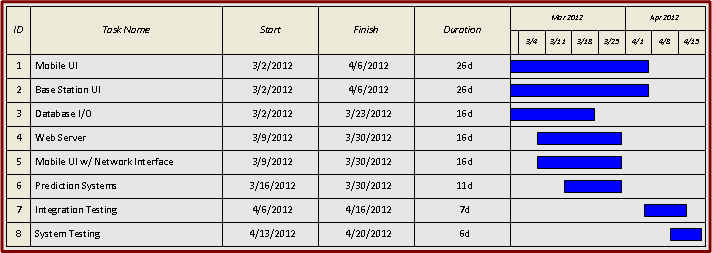
\includegraphics[scale=.6]{GanttChartI}
\end{center}
\end{figure}

\end{document}
